% GENERATED by scripts/build_paper.py from body.template.tex; edit the template, never this file.
% SOURCE of the paper body, shared by main_single.tex and main_twocol.tex. Numbers are never typed here: every
% double-brace placeholder is filled by scripts/build_paper.py from results/paper_numbers.json, which
% scripts/paper_numbers.py, air_numbers.py, revision_numbers.py, s1_numbers.py and rw_numbers.py read from result files.
\title{One Step Ahead Is Not Enough: Testing a Learned Quadruped Simulator at the Horizon It Is Used}
\author{\anonauthor}
\maketitle

\begin{abstract}
Learned simulators let legged robots learn in long imagined rollouts, yet are often trained, compressed and checked
one step ahead. We rebuilt the open quadruped simulator of the Robotic World Model (RWM) and measured 101
trained simulators and 200 compressed copies. One-step checks picked the wrong training choices: teacher
forcing and one-step training were better one step ahead but 2.0 and 2.6 times as wrong
at 2~s (descriptive; partly registered earlier), also after longer training and in two of three other architectures.
Pruning 30\% of weights kept 90\% of the skill one step ahead, 39\% at 2~s (descriptive);
fine-tuning restored nearly all of it (registered). The error growth rate, needing no recorded future, ranked
simulators by 2-second error better than one-step error (registered) on 97 GRU simulators and, averaged, over
three other architectures (two carry it). On the GRU pool it was not separated from 8-step error
(registered) and failed a secondary replication on mostly compressed copies. A kinematic residual ranked them
best with recorded commands (descriptive; its lead over 8-step error failed multiple-test correction), and less
well under RWM's policy (registered). Scope: simulated data, one robot and trotting
gait, no physics-simulator test.
\end{abstract}

\begin{IEEEkeywords}
learned simulators, world models, legged robots, model-based reinforcement learning, Lyapunov exponents,
model compression, uncertainty
\end{IEEEkeywords}

\section{Introduction}\label{sec:intro}
A legged robot can learn to walk inside a \emph{learned simulator}: a neural network that predicts the robot's next
state from its recent states and \emph{joint commands} (the 12 joint position targets given at every step), run
forward on its own predictions, as image-based world models are~\cite{hafner2025}. Such a run is a \emph{rollout},
and its length is its \emph{horizon}; because each prediction becomes the next input, small errors can
grow~\cite{venkatraman2015,talvitie2017,lambert2022compounding,janner2019}. The Robotic World Model
(RWM)~\cite{li2025rwm} learns such a simulator for an ANYmal~D quadruped and imagines 24 steps per policy update;
RWM-U~\cite{li2025rwmu} trains a walking policy inside 100-step imagined rollouts. RWM trains on its own 8-step
rollouts; its ablation found this better than teacher forcing, and the forecast horizon decisive for long-term
accuracy~\cite[Sec.~4.3, App.~A.4.1]{li2025rwm}.

Elsewhere, one-step checks remain common. Offline model-based methods build on ensembles of one-step
models~\cite{yu2020mopo,yu2021combo}, and RAMBO keeps the members with the lowest error on held-out single
transitions~\cite{rigter2022rambo}. Compression~\cite{han2016} and uncertainty estimates~\cite{chua2018,yu2020mopo}
are judged one step at a time, although one-step accuracy need not track what a model is used
for~\cite{lambert2020objective}. We ask two questions. \emph{When does a one-step check give the wrong answer about a
simulator used 100 steps ahead?} And \emph{can a cheap check that needs no recorded future states do better?}

We answer on RWM's open-source dynamics model, in a narrow setting: one robot, one trotting gait on flat ground,
simulated data, and no test of a trained policy in a physics simulator. We rebuilt the model, matched the release's
gradients exactly, and measured 101 trained simulators and 200 compressed copies. Every
comparison of checks was registered before its measurements were run. Our first two results independently confirm
RWM's ablation; we add the one-step view, other architectures and a policy in the loop. Our contributions are:
\begin{itemize}
\item \textbf{Where one-step checks mislead} (Sec.~\ref{sec:decisions}): judged one step ahead, teacher forcing,
one-step training and pruning without retraining look better or nearly harmless; at the horizon of use they are worse. The
reversal persists after four times longer training and in two of three other architectures, and fine-tuning repairs
the pruned copies (registered).
\item \textbf{A registered comparison of checks that need no recorded future} (Sec.~\ref{sec:checks}): the growth
rate of small errors and a kinematic residual against one-step and 8-step error, on two pools of RWM-style simulators,
three other architectures and two sources of joint commands.
\item \textbf{A checklist} for vetting a learned simulator before long imagined rollouts (Sec.~\ref{sec:discussion}).
\end{itemize}

\section{Related Work}\label{sec:related}
\textbf{Compounding error.} Training on a model's own
predictions~\cite{bengio2015scheduled,venkatraman2015,talvitie2017,lambert2021} and limiting rollout
length~\cite{janner2019} are established remedies for errors that grow along a rollout; one-step likelihood need not
track control performance (\emph{objective mismatch}~\cite{lambert2020objective}).
\textbf{Uncertainty for model-based control.} Ensembles~\cite{lakshminarayanan2017,chua2018} estimate uncertainty;
offline methods keep the members with the lowest held-out one-step error~\cite{rigter2022rambo}, penalise imagined
reward by their disagreement~\cite{yu2020mopo,li2025rwmu}, and compare penalties by how well they track
error~\cite{lu2022}; recalibration corrects predicted uncertainty on held-out
data~\cite{kuleshov2018accurate,malik2019calibrated}.
\textbf{Stability of recurrent networks.} Products of Jacobians govern exploding
gradients~\cite{pascanu2013difficulty}; contracting recurrent models are easier to train~\cite{miller2019stable};
Lyapunov spectra characterise chaotic recurrent networks~\cite{engelken2024lyapunov} and their training difficulty,
which modified teacher forcing addresses~\cite{mikhaeil2022chaotic,hess2023generalized}; stable dynamics can be
learned by construction~\cite{manek2019stable}.
\textbf{Physics and compression.} Kinematic consistency has diagnosed long-horizon failure of imagined
rollouts~\cite{schafer2026}, like parity relations~\cite{isermann2005}; compressed world models are judged by task
success~\cite{fu2026} or error growth~\cite{pavlova2026}, and pruning is often matched by small networks trained from
scratch~\cite{liu2019rethinking}.

\section{System and Protocol}\label{sec:setup}
\textbf{Data.} The release contains 10{,}000 recorded steps of an ANYmal~D trotting on flat ground at 50~Hz: ten
20-second episodes, in each of which the \emph{velocity command} (the walking speed and turning rate the robot is
asked to follow) appears to change once. Every episode starts from an exact reset, so the data come from a physics
simulation, not the hardware. Each step holds a 45-number state (body velocities, the direction of gravity seen from
the body, and each joint's angle, speed and torque) and the 12 joint commands. These data are 0.13\% of what
the original model was trained on.

\textbf{Simulator and rebuild.} The network is RWM's: two layers of gated recurrent units (GRU, a standard recurrent
layer) of width 256 read the last 32 states and joint commands and predict the change to the next state. RWM trains it
on its own 8-step rollouts (\emph{rollout training}); its released checkpoint has five output heads on one shared
trunk, whose spread is the uncertainty RWM-U uses. Our rebuild reproduces the release's outputs bit for bit and its
gradients exactly, and avoids two defects of the release: training windows spliced across episodes, and evaluation
commands fed one step late (appendix~A1).

\textbf{Held-out data and pools.} Each held-out episode yields two non-overlapping trajectories of 32 history and 368
forecast steps (7.36~s). The \emph{main pool} (F18) holds out episodes 1 and 8 (four trajectories) and has 97
simulators. The \emph{five-split pool} (X5) holds each episode out once (20 trajectories, 255 simulators, each
scored on its own split).

\textbf{Models.} The main pool has 48 rollout-trained models: five seeds of the released configuration (history
$M=32$, training horizon $N=8$) and variants such as ensembles, a likelihood loss and other $(M,N)$ settings. 9
were trained one step ahead, by \emph{teacher forcing}~\cite{williams1989} (each step predicted from the true previous
state, never from the model's own prediction) or with $N=1$. The other 40 are compressed copies, made after
training: weights rounded to 16 or 8 bits, the smallest 10--50\% of weights set to zero (\emph{pruning}), or GRU units
removed. The five-split pool repeats the main training methods and compressions on every split. The main pool also holds
teacher-forced and rollout-trained models trained four times longer, and study AR used 38 simulators of three
other architectures trained on F18's split. Training used the release's loss and Adam for 2{,}500 iterations unless stated, on a
CPU (appendix~A1).

\textbf{Measures.} Error is the mean absolute error over the 45 state numbers, each divided by its standard deviation
in the data. $E_h$ is the mean error over $h$-step rollouts started, after 32 true history steps, from every fourth
held-out position ($E_1$: every position); $E_{368}$ uses one 368-step rollout per trajectory. The \emph{floor}
predicts no change, holding the last history state. A compressed copy's \emph{skill retained} is $K(h)=1-\Delta(h)/S(h)$,
where $\Delta$ is its extra error over its parent and $S$ the parent's advantage over the floor; $K<0$ is worse than
predicting no change. Two checks are \emph{label-free}: they need the history and the joint commands but no recorded
future state. The \emph{growth rate} $\lambda_1$, the leading finite-time Lyapunov exponent, is the average
exponential rate per second at which the gap between two copies of the simulator, started from almost identical
internal states and given the same joint commands, grows ($\lambda_1>0$) or shrinks ($<0$, a \emph{contracting}
simulator); we compute it over each 368-step rollout by Benettin's method~\cite{benettin1980}. The \emph{kinematic
residual} $\bar r_J$ asks whether predicted joint angles change as the predicted joint speeds say, each joint in units
of its residual in the training episodes, averaged over the rollout.

\textbf{Statistics and registration.} Intervals are 95\% percentile intervals from 20{,}000 bootstrap draws over
the independent unit: whole trajectories for comparisons of methods~\cite{cameron2008,agarwal2021}, models for
correlations. A result is \emph{registered} if its decision rule was committed to version control before the
measurements that test it were run~\cite{nosek2018prereg}; a rule gives a verdict only when its interval clears a stated threshold
(usually zero), and ``not settled'' otherwise. Three registrations were made for this paper: the comparison of checks
on both pools (primary Q1--Q2, secondary Q3--Q6), study FT on fine-tuning pruned copies (FT1--FT2), and studies CL
and AR on policy commands and other architectures (CL1--CL2, AR1--AR2). Primary questions are judged at 97.5\%. Two parts of the
first were known from earlier analyses (appendix~A2). Other verdicts come from rules registered for earlier,
unpublished analyses; those registrations and all code are in the anonymised supplementary material. Secondary
verdicts are judged at 95\% without correction; Holm's correction over the 7 secondary tests of Q3--Q6
is exploratory. Everything else is descriptive, or exploratory where it was added after the registered results were
seen. Resampling parents and trajectories together widens the intervals on correlations by a median factor of
1.5 (exploratory, appendix~A4).

\section{Results}\label{sec:results}
\subsection{One-step checks reverse training and compression choices}\label{sec:decisions}
Table~\ref{tab:decisions} judges each choice one step ahead and at 24, 100 and 368 steps (0.48, 2 and 7.4~s); RWM
and RWM-U imagine 24 and 100 steps.

\begin{widetable}[t]
\centering
\caption{Each choice judged one step ahead and at longer horizons. Error ratio: error of the one-step-trained model
(teacher-forced, or $N{=}1$) over the 8-step rollout-trained model's; above 1, the one-step choice is worse. Skill
retained $K$: the share of the parent's advantage over predicting no change that the copy keeps (${<}0$: worse than
no change). Spread factor: how many times the released ensemble's spread must grow to cover 68\% of outcomes (--: not
computed). Fine-tuned row: seeds 0--2 of each split. Last column: models; held-out trajectories.}
\label{tab:decisions}
\footnotesize
\setlength{\tabcolsep}{3.5pt}
\fittable{\begin{tabular}{@{}llccccl@{}}
\toprule
Choice & Measure & 1 step & 24 steps & 100 steps & 368 steps & Models, trajectories \\
\midrule
Training objective & error ratio, teacher-forced / rollout & 0.90 & 1.5 & 2.0 & 5.0 & 40 on X5, 20 \\
Training horizon & error ratio, $N{=}1$ / $N{=}8$ & 0.86 & 1.8 & 2.6 & 5.4 & 8 on F18, 4 \\
\midrule
8-bit weights & skill retained $K$ & 99.7\% & 99.3\% & 97.0\% & 95\% & 25 + 25 on X5, 20 \\
Pruning 20\% of weights & skill retained $K$ & 97.4\% & 95\% & 80\% & 57\% & 25 + 25 on X5, 20 \\
Pruning 30\% of weights & skill retained $K$ & 90\% & 83\% & 39\% & $-$41\% & 25 + 25 on X5, 20 \\
Pruning 30\%, then fine-tuned for 500 iterations & skill retained $K$ & 102.3\% & 100.9\% & 102.2\% & 103.9\% & 15 + 15 on X5, 20 \\
\midrule
Ensemble uncertainty & spread factor & 6.6 & -- & 30.8 & 41.7 & released, 20 \\
\bottomrule
\end{tabular}}
\end{widetable}

\begin{widefigure}[t]
\centering
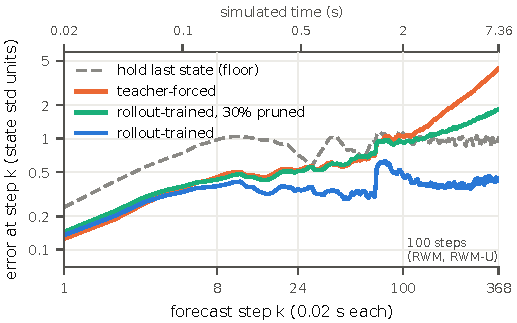
\includegraphics[width=\figw]{figures/fig_horizon.pdf}
\caption{Error at each forecast step on the 20 held-out trajectories of the five splits (models averaged within each
trajectory). Teacher forcing first exceeds the floor (holding the last state) at step 29, the 30\%-pruned
copy at step 57. Vertical lines: the imagination horizons of RWM and RWM-U.}
\label{fig:horizon}
\end{widefigure}

\textbf{Training objective and horizon.} The first two rows confirm RWM's ablation~\cite{li2025rwm} on
0.13\% of its data: rollout training beats teacher forcing at the horizon of use, and a longer training
horizon helps. One step ahead the order is reversed: teacher forcing's one-step error is 10\% lower
(descriptive), as an earlier registered analysis also found. By 8 steps teacher forcing is worse on 19
of the 20 trajectories, and the gap grows with the horizon (Fig.~\ref{fig:horizon}); at 368 steps an earlier registered
rule found rollout training better on all 10 held-out episodes. Over 2~s the teacher-forced simulator's
joint angles are off by 7.0$^\circ$, against 3.4$^\circ$ (body position: appendix~A1).
Training with $N=1$ shows the same reversal.

Longer training and other networks test whether the reversal is specific to this setup (descriptive). Trained four
times longer,
teacher forcing was still better one step ahead and worse at 100 steps in each of 3 seeds, while the
training loss was still falling in 5 of 6 runs (appendix~A10). The
teacher-forced run was better one step ahead and worse at 100 steps in 5 of
5 seed pairs of an MLP simulator and 5 of
5 of a Transformer. In an RSSM (a recurrent state-space model), it was better one step
ahead in 5 of 5 pairs but worse at 100 steps in
0 of them (appendix~A9).

\textbf{Stability.} The growth rate tracks the training horizon: it is positive for $N=1$ (+0.61/s) and falls
through +0.44, $-$0.43 and $-$1.13 to $-$1.38/s at $N=32$ (descriptive; a rule committed before that
analysis found the same order, appendix~A1). Every rebuilt model trained on its own rollouts of eight or more steps
was contracting, and no teacher-forced one was. The released model does not fit: trained on about 750 times
more data, it has $\lambda_1={}$+0.70/s on these trajectories, which it may have trained on (appendix~A6). The
account therefore covers only models trained on this data set.

\textbf{Compression.} Pruning 30\% of weights without retraining keeps 90\% of the parent's skill one step
ahead but 39\% at 100 steps, and by 368 steps the copy is worse than predicting no change (descriptive). In
a registered follow-up (appendix~A7), 500 iterations of fine-tuning with the pruned weights held at zero restored the
100-step skill from 38\% to 102.2\% (\textsc{fine-tuning restores skill}); the fine-tuned copies were
\textsc{nearly as skilled} as their parents fine-tuned the same way (99.9\% [99.5\%, 100.4\%]). Skill above
100\% mostly reflects the extra training, not the pruning (descriptive). Moderate pruning adds error but barely moves the growth
rate: at 30\% the registered test could not separate the shift (+0.03/s [$-$0.02, +0.07]) from zero
(\textsc{not settled}; secondary), and no copy pruned by 10--30\% has $\lambda_1>0$ (appendix~A5). Rounding weights
to 8 bits keeps 97.0\% of the 100-step skill (descriptive; weights only).

\textbf{Uncertainty} (descriptive). The released ensemble's spread ranks error well (Spearman +0.90 with
the 100-step error, on episodes it may have trained on) but is too narrow, by a factor of 6.6 one step ahead and
30.8 at 100 steps, so a one-step calibration check understates the problem. Each head's own variance collapses,
because the implemented loss is smallest at zero variance (appendix~A6).

\subsection{Which check ranks simulators without recorded futures?}\label{sec:checks}
A label-free check could vet a simulator on new velocity commands, or while a policy drives it. The main registered
comparison and studies AR and CL asked whether $\lambda_1$ and $\bar r_J$ rank simulators by their 100-step error $E_{100}$ better than the labelled
one-step and 8-step errors $E_1$ and $E_8$. Table~\ref{tab:checks} gives the correlations, Table~\ref{tab:verdicts}
the registered verdicts.

\begin{widetable}[t]
\centering
\caption{Spearman correlation of each check with the 100-step error $E_{100}$ under recorded commands, across
simulators (number in brackets). F18, main pool: checks computed with recorded or with the policy's joint commands.
X5: within each split, averaged. Other architectures: F18's split, within each architecture. Closed loop: $\lambda_1$
with the policy differentiated too. --: not applicable. E: exploratory. Correlations are descriptive;
Table~\ref{tab:verdicts} gives the registered tests.}
\label{tab:checks}
\footnotesize
\setlength{\tabcolsep}{4pt}
\fittable{\begin{tabular}{@{}lccccccc@{}}
\toprule
 & Needs recorded & F18, recorded & F18, policy & X5 & MLP & RSSM & Transformer \\
Check & future states & (97) & (97) & (255) & (13) & (12) & (13) \\
\midrule
One-step error $E_1$ & yes & +0.32 & -- & +0.78 & $-$0.69 & +0.88 & $-$0.61 \\
8-step error $E_8$ & yes & +0.84 & -- & +0.95 & +0.76 & +0.86 & +0.73 \\
Growth rate $\lambda_1$ & no & +0.80 & +0.76 & +0.67 & +0.84 & +0.26 & +0.87 \\
\quad closed loop & no & -- & $-$0.01 & -- & -- & -- & -- \\
Kinematic residual $\bar r_J$ & no & +0.95 & +0.83 & +0.96 (E) & +0.76 & +0.94 & +0.98 \\
\bottomrule
\end{tabular}}
\end{widetable}

\begin{table}[t]
\centering
\caption{Registered verdicts. Estimate: difference in Spearman correlation with $E_{100}$, first check minus second
(CL: policy minus recorded joint commands); FT1: gain in skill retained at 100 steps, in points; FT2: skill retained
against a parent fine-tuned the same way. AR: the three other architectures, averaged. P: primary, 97.5\% interval; S: secondary, 95\%. $^\dagger$: fails Holm's
correction (exploratory).}
\label{tab:verdicts}
\footnotesize
\setlength{\tabcolsep}{2pt}
\begin{tabular}{@{}llllp{2.5cm}@{}}
\toprule
 & Comparison & Pool & Estimate & Verdict \\
\midrule
Q1 P & $\lambda_1$ vs $E_1$ & F18 & +0.48 [+0.20, +0.79] & \textsc{label-free better} \\
Q2 P & $\lambda_1$ vs $E_8$ & F18 & $-$0.04 [$-$0.20, +0.14] & \textsc{not settled} \\
Q3 S & $\lambda_1$ vs $E_1$ & X5 & $-$0.12 [$-$0.22, $-$0.03]$^\dagger$ & \textsc{one-step better} \\
Q3 S & $\lambda_1$ vs $E_8$ & X5 & $-$0.28 [$-$0.37, $-$0.22] & \textsc{training-horizon better} \\
Q4 S & $\bar r_J$ vs $E_1$ & F18 & +0.63 [+0.41, +0.88] & \textsc{label-free better} \\
Q4 S & $\bar r_J$ vs $E_8$ & F18 & +0.12 [+0.02, +0.23]$^\dagger$ & \textsc{label-free better} \\
AR1 P & $\lambda_1$ vs $E_1$ & AR & +0.796 [+0.368, +1.025] & \textsc{label-free better} \\
AR2 P & $\bar r_J$ vs $E_8$ & AR & +0.110 [$-$0.081, +0.356] & \textsc{not settled} \\
CL1 P & $\bar r_J$, policy & F18 & $-$0.120 [$-$0.220, $-$0.052] & \textsc{worse with policy commands} \\
CL2 P & $\lambda_1$, policy & F18 & $-$0.032 [$-$0.113, +0.041] & \textsc{not settled} \\
FT1 P & fine-tuned & X5 & +63.9 [54.4, 76.0] & \textsc{fine-tuning restores skill} \\
FT2 P & fine-tuned & X5 & 99.9\% [99.5\%, 100.4\%] & \textsc{nearly as skilled} \\
\bottomrule
\end{tabular}
\end{table}

\textbf{Main pool, recorded commands.} Across the 97 simulators of the main pool (Fig.~\ref{fig:checks}),
one-step error ranked the 100-step error poorly (+0.32) and the growth rate well (+0.80). The first
primary question found the growth rate better (\textsc{label-free better}). The second could not separate it from the
8-step error (\textsc{not settled}), which ranked ahead of it at 24 steps (secondary). Models trained one step
ahead have among the lowest one-step but high 100-step errors, and one-step error ranks the 57 trained
models backwards ($-$0.50; exploratory); every check ranks the compressed copies well (appendix~A4). The
kinematic residual ranked best (+0.95; descriptive). The registered rules favoured it over both $E_1$ and
$E_8$ (secondary), but only its lead over $E_1$ survives Holm's correction (exploratory).

\textbf{Five-split pool.} The registered replication on the five-split pool, where most of the 51
simulators per split are compressed copies, failed for the growth rate: one-step error ranked better than it
(\textsc{one-step better}; secondary), and the 8-step error better still. The first reading is not resolved under
the wider intervals, but the growth rate did not beat one-step error in any reading (exploratory, appendix~A4). The likely cause
is that moderate pruning adds error while barely changing the growth rate, so a negative growth rate certifies
nothing: of the 17 main-pool simulators worse than the floor at 100 steps, 15
had $\lambda_1\le0$. The kinematic residual, registered on the main pool only, was level with the 8-step error here
(+0.01 [$-$0.01, +0.03]; exploratory).

\textbf{Other architectures.} Study AR repeated the two comparisons that had favoured the label-free checks on
38 runs of an MLP, an RSSM and a Transformer simulator, ranking within each architecture and averaging. AR1
found the growth rate better than one-step error (\textsc{label-free better}), carried by the MLP and the Transformer,
where one-step error ranked the runs largely in reverse. In the RSSM, one-step error ranked them better
(+0.88 against +0.26; descriptive). AR2, the residual against the 8-step error, was
\textsc{not settled}. Ranked across architectures together, neither comparison was settled and the growth rate
did not rank the runs ($\rho={}$$-$0.11); with the main pool added, AR1 was
\textsc{label-free better} (both secondary).

\textbf{Policy commands.} Study CL let the RWM authors' released policy, not the recording, supply the joint commands:
at each step it read the simulator's own predicted state and a fixed velocity command. Such a rollout has no recorded
future, so the checks were ranked against $E_{100}$ under recorded commands. The residual then ranked less well
(\textsc{worse with policy commands}; +0.83 against +0.95), a drop carried by the trained models
(secondary) and seen again on the five-split pool (secondary). The growth rate's change was \textsc{not settled}.
With small noise added to the recorded commands instead, both checks were \textsc{unchanged by the command source} (within $\pm$0.10; secondary).
Differentiated through the policy as well (closed loop), the growth rate was \textsc{worse with policy commands}
(secondary) and did not rank the simulators ($\rho={}$$-$0.01). Simulators with higher error gave the policy lower imagined return
($\rho={}$$-$0.86; secondary), and none of the 352 GRU simulators diverged under policy,
closed-loop or noisy commands (descriptive).

\begin{widefigure}[t]
\centering
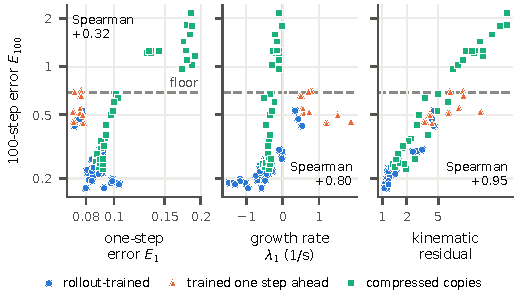
\includegraphics[width=\figw]{figures/fig_checks.pdf}
\caption{One-step error, growth rate and kinematic residual (left to right) against 100-step error for the 97
simulators of the main pool. Models trained one or two steps ahead have low one-step but high 100-step errors, and
positive growth rates; compressed copies (squares) spread vertically at nearly constant growth rate. Dashed: the
floor.}
\label{fig:checks}
\end{widefigure}

\stepslot

\section{Discussion}\label{sec:discussion}
\textbf{Why one-step checks mislead here.} A one-step check feeds a simulator true recorded states, inputs it never
produces itself. In use it reads its own predictions, so what matters is how it treats its own errors. Teacher forcing
and one-step training never show the network those errors, and the simulators they produced amplify them
($\lambda_1>0$). Pruning without retraining appears to add a small error at each step that accumulates over the rollout. One-step
error therefore ranked training choices backwards, while it ranked copies of the same parent well.

\textbf{A checklist from this case study.} (1)~\emph{Train and validate at the horizon of use}, on held-out
episodes, counting independent trajectories. (2)~\emph{Fine-tune after pruning}, and check the pruned copy at the
horizon of use. (3)~\emph{Without recordings, screen with label-free checks and know their limits}: the residual
ranked RWM-style simulators best with recorded commands but less well under a policy; a positive growth rate flagged
the one-step-trained simulators, a negative one certifies nothing, and growth rates did not rank different
architectures together. (4)~\emph{Read ensemble spread as a ranking}; rescale it per horizon on held-out episodes
before using it as an interval, and do not rely on label-free run-time alarms, which lost to a step counter or a fixed
schedule in earlier registered analyses (appendix~A6).

\textbf{Limitations.} All evidence comes from one robot, one trotting gait on flat ground and ten 20-second episodes
of simulated data, so ``held out'' means other velocity commands of the same gait. The policy drove the simulators
only in imagination: no policy was trained, and nothing was tested in a physics simulator or on hardware, so what a
mis-ranked simulator costs a controller is not measured, and imagined return is not walking performance. Under policy
commands the checks are compared with error under recorded commands. The main pool has four held-out trajectories,
which bounds every interval. Correlations treat models as independent although they share parents, data and test
trajectories; wider intervals that allow for this leave 3 of 13 registered verdicts
unresolved (exploratory). The growth rate is a finite-time exponent in the network's own coordinates, and the
stability account does not cover the released model. Each other architecture has 12 or
13 runs, and the longer-training check has 3 seeds and no intervals.

\section{Conclusion}\label{sec:conclusion}
On this simulator, one-step checks favoured teacher forcing, one-step training and a pruned model that, without
fine-tuning, loses most of its skill by 2~s. Without recorded futures, on the main pool the growth rate ranked RWM-style
simulators better than one-step error but was not separated from 8-step error, and a negative value certifies nothing; the
kinematic residual ranked them best with recorded commands and less well under a policy. Whether these checks predict
how well a policy trained inside the simulator walks is the next question.

\textbf{Reproducibility and use of AI tools.} The registrations and code are in the
supplementary material. An AI assistant (Claude, Anthropic), directed by the author(s), wrote
analysis code, ran analyses and drafted text; the author(s) are responsible for the content.

\bibliographystyle{IEEEtran}
\bibliography{refs}
